The given information is available in 
\tabref{tab:chapters/11/11/4/13/1}.
Since two foci are given, the conic cannot be a parabola.
\begin{enumerate}
\item The direction vector of $F_1F_2$ is the normal vector of the directrix.  Hence, 
\begin{align}
\vec{n} = \vec{F_1} - \vec{F_2}
	\equiv \vec{e}_1
\end{align}
Substituting in 
  \eqref{eq:conic_quad_form_v},
\eqref{eq:conic_quad_form_u}
and
\eqref{eq:conic_quad_form_f},
\begin{align}
	\vec{V} &= \myvec{1-e^2&0\\0&1} \label{eq:chapters/11/11/4/13/6} 
	\\
	\vec{u} &= ce^2\vec{e}_1-\vec{F}
\label{eq:chapters/11/11/4/13/6/u} 
	\\
	f&=16-c^2e^2
\label{eq:chapters/11/11/4/13/6/f} 
\end{align}
\item From
\eqref{eq:chapters/11/11/4/13/6},
\begin{align}
\lambda_1 &= 1-e^2,\
\lambda_2 = 1
\label{eq:chapters/11/11/4/13/12}
\end{align}
which upon substituting
in
			\eqref{eq:latus-ellipse}, along with the value of the latus rectum 
from \tabref{tab:chapters/11/11/4/13/1}
		\begin{align}
	6\brak{1-e^2} = \sqrt{\abs{f}}
\label{eq:chapters/11/11/4/13/12/f}
\end{align}
\item  The centre of the conic is given by
\begin{align}
\vec{c} = \frac{\vec{F_1} + \vec{F_2}}{2}
= \vec{0}
\label{eq:chapters/11/11/4/13/5}
\end{align}
From \eqref{eq:chapters/11/11/4/13/6}, it is obvious that  
$\vec{V}$ is invertible.  Hence,  
from \eqref{eq:chapters/11/11/4/13/5}
and 
\eqref{eq:conic_parmas_c_def},
\begin{align}
\vec{u} = \vec{0}
	\label{eq:chapters/11/11/4/13/7/u}
\end{align}
Substituting the above in \eqref{eq:chapters/11/11/4/13/6/u}, 
\begin{align}
\vec{F} = ce^2\vec{e}_1 
\implies 
	\norm{\vec{F}} = 4 = ce^2
	\label{eq:chapters/11/11/4/13/7}
\end{align}
\item 
	From 
      \eqref{eq:f0}, 
	\eqref{eq:chapters/11/11/4/13/7/u}
and
\eqref{eq:chapters/11/11/4/13/6/f},
		\begin{align}
	36\brak{1-e^2}^2 = 16-c^2e^2
\label{eq:chapters/11/11/4/13/12/ec}
\end{align}
From
	\eqref{eq:chapters/11/11/4/13/7}
	and
\eqref{eq:chapters/11/11/4/13/12/ec}
\begin{align}
\frac{4}{e\sqrt{e^2-1}} &= 6
\\
\implies 9e^2\brak{e^2-1} &= 4\\
\implies 9e^4-9e^2-4 &= 0
\\
	\text{or, }\brak{3e^2-4}
	\brak{12e^2+1} &=0
\label{eq:chapters/11/11/4/13/14}
\end{align}
yielding
\begin{align}
e = \frac{4}{3}
\end{align}
as the only viable solution.
\end{enumerate}
The equation of the conic is then obtained as
\begin{align}
\vec{x}^\top\myvec{-\frac{1}{3}&0\\0&1}\vec{x} +4 = 0
\end{align}
See \figref{fig:chapters/11/11/4/13/1}.
\begin{figure}[H]
\centering
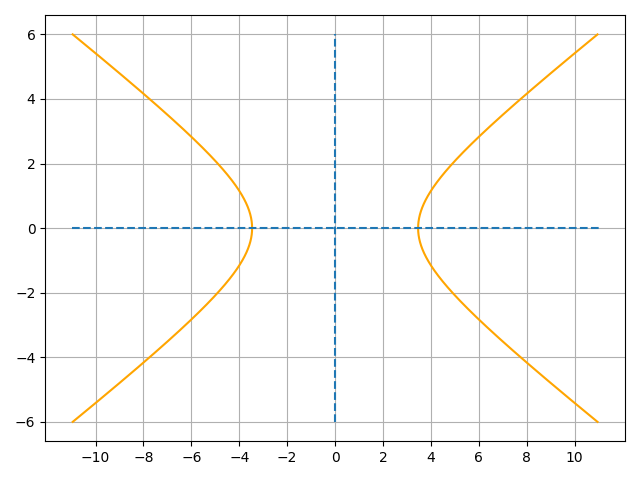
\includegraphics[width=0.75\columnwidth]{chapters/11/11/4/13/figs/fig1.png}
\caption{}
\label{fig:chapters/11/11/4/13/1}
\end{figure}
\begin{table}[H]
\centering
\begin{tabular}{|p{3cm}|p{3cm}|p{3cm}|}
\hline                                        
\textbf{Symbol} & \textbf{Values} & \textbf{Description}\\                                          
\hline                                 
$\theta$ & 30$\degree{}$   & $\angle{BAD} = \angle{BAC}$ \\           
\hline                                    
a &  9 & $AB$ \\     
\hline                      
c & 5 & $AC$ \\
\hline                                     
		$\vec{e}_1$ & $\myvec{
			1\\
			0\\
			}$ & basis vector\\ 
\hline
\end{tabular}

\caption{}
\label{tab:chapters/11/11/4/13/1}
\end{table}
